\documentclass[sigconf, nonacm]{acmart}

%%% do not modify the following VLDB block %%%
%%% VLDB block start %%%
\usepackage{pvldb}
%%% VLDB block end %%%

\renewcommand\vldbdoi{XX.XX/XXX.XX}
\renewcommand\vldbpages{XXX-XXX}
\renewcommand\vldbavailabilityurl{https://github.com/CKTtari/maximal-semantic-clique-enumeration}

\usepackage[linesnumbered,ruled,vlined]{algorithm2e}
\usepackage{amsmath,amsfonts}
\usepackage{algorithmic}
\usepackage{enumitem}

\usepackage{tikz}
\usetikzlibrary{arrows.meta,decorations.pathreplacing}
\usepackage{pgfplots}
\usepgfplotslibrary{statistics}
\usepackage{xcolor}
\usepackage{colortbl}
\definecolor{bestgreen}{HTML}{DCEFE2}
\definecolor{midyellow}{HTML}{FFF1BF}
\definecolor{accentblue}{HTML}{DCEAF7}
\definecolor{accentred}{HTML}{F6D7DB}
\pgfplotsset{compat=1.17}
\usepackage{amsthm}
\usepackage{multirow}
\usepackage{subcaption}
\usepackage{placeins}
\newtheorem{problem}{Problem}

\newtheorem{definition}{Definition}
\newtheorem{example}{Example}
\newtheorem{observation}{Observation}[section] 
\newtheorem{corollary}{Corollary }[section]
\newtheorem{theorem}{Theorem}[section]
\newtheorem{lemma}{Lemma}[section]
\newtheorem{property}{Property}[section]
%\newenvironment{proof}{ {\it  Proof:} }{\hfill $\square$\par}  


\newcommand{\kw}[1]{{\ensuremath {\mathsf{#1}}}\xspace}
\newcommand{\kwnospace}[1]{{\ensuremath {\mathsf{#1}}}}
\newcommand{\stitleunderline}[1]{\vspace{0.7ex}\noindent\underline{{\bf #1}}}
%\newcommand{\stitleunderline}[1]{\vspace{1ex} \noindent{\bf #1}}
\newcommand{\stitle}[1]{\vspace{0.7ex} \noindent{\bf #1}}
\long\def\comment#1{}
\newcommand{\eop}{\hspace*{\fill}\mbox{$\Box$}}
\newcommand{\eopfill}{\hfill{\rule[0pt]{1.3ex}{1.3ex}}}
\def\done{\hspace*{\fill}$\square$\par}

%% ---------------------------------------------------------------
%% Unified notation macros (single source of truth)
%%
%%   \avgsim(C)   闂?average pairwise similarity of clique C
%%                  = (2 / |C|(|C|-1)) * sum_{u<v in C} sim(u,v)
%%
%%   \simsum(C)   闂?total pairwise similarity sum of clique C
%%                  = sum_{u<v in C} sim(u,v)
%%
%%   \W(C)        闂?semantic surplus of clique C w.r.t. threshold tau
%%                  = simsum(C) - tau * C(|C|,2)  (positive iff avgsim >= tau)
%%
%%   \acc[v]      闂?accumulated similarity of candidate v to current clique C
%%                  = sum_{u in C} sim(u,v)
%%
%%                  = avgsim(C) * C(|C|+1,2) - simsum(C)
%% ---------------------------------------------------------------
\newcommand{\StructBK}{\textsc{Struct\-BK}}
\newcommand{\semBK}{\textsc{SemBK}}
\newcommand{\subEnum}{\textsc{StrSub}}
\newcommand{\monoSemMCE}{\textsc{Mono\-Sem\-MCE}}
\newcommand{\pairSim}{\textsc{PairSim-MCE}}
\newcommand{\avgsim}{\mathrm{avgSim}}
\newcommand{\simsum}{\mathit{simSum}}
\newcommand{\W}{\mathit{W}}
\newcommand{\acc}{\mathit{acc}}


\begin{document}
\title{Maximal Semantic Clique Enumeration in Vector-Attributed Graphs}
%%
%% The "author" command and its associated commands are used to define the authors and their affiliations.
\author{Tianyi Gao}
\affiliation{%
  \institution{Beijing Institute of Technology}
  \city{Beijing}
  \country{China}
}
\email{tygao\_bit@163.com}

\author{Hongchao Qin}
\affiliation{%
  \institution{Beijing Institute of Technology}
  \city{Beijing}
  \country{China}
}
\email{qhc\_neu@gmail.com}

%%
%% The abstract is a short summary of the work to be presented in the
%% article.
\begin{abstract}
Vector-attributed graphs encode two complementary forms of group cohesion:
edges record structural relations, while vertex vectors describe semantic
compatibility. Maximal clique enumeration captures the former but provides no
criterion for the latter. We study maximal semantic clique (MSC) enumeration,
which retains complete connectivity and requires the average pairwise vector
similarity to reach a threshold. Unlike an every-pair threshold, this aggregate
criterion tolerates a small number of atypical pairs when the group remains
collectively coherent. It is also non-monotone over clique containment, so
structural pivot pruning and early rejection of infeasible partial cliques are
not directly applicable. We propose two efficient algorithms with different
advantageous regimes under this constraint. \subEnum\ restores structural pivoting by
separating structural MCE from bounded semantic subset enumeration.
\monoSemMCE\ uses a feasible-parent theorem: deleting a deterministic
minimum-contribution vertex from any feasible clique preserves feasibility.
The induced canonical forest generates each feasible state once without a
visited table or materialized size layers. Across three naturally attributed
and five controlled vector-attributed graphs, the two specialized methods
jointly complete all 24 workloads, whereas the \semBK\ baseline reaches
the 1,200-second limit on 15. At $q_{99}$, \monoSemMCE\ is
$2.92\times$--$6.24\times$ faster than \subEnum. On two real graphs,
pairwise-threshold MCE retains no reference MSC of size at least ten on GitHub-Social and
only 0.32\% on ogbn-arxiv-25K, demonstrating the model-level fragmentation
avoided by the average constraint.
\end{abstract}
\maketitle

%%% do not modify the following VLDB block %%
%%% VLDB block start %%%
\vldbtopmatter
%%% VLDB block end %%%

\section{Introduction}
\label{sec:intro}

Graphs with vector-valued attributes are increasingly common in data management:
social networks associate users with profile features, knowledge graphs attach
text embeddings to entities, and citation graphs represent papers by content
vectors~\cite{rozemberczki2021musae,toutanova2015observed,wang2020ogb}.
Existing models combine dense structure with attributes through
correlated patterns and similarity-constrained bipartite
subgraphs~\cite{silva2012,yao2022similarbiclique}. These tasks expose a basic modeling
gap: adjacency establishes interaction, whereas vector similarity establishes
semantic compatibility, and neither signal alone identifies groups satisfying
both requirements.

The maximal clique is the strongest structural model of cohesion: every pair of
vertices is connected. In a vector-attributed graph, this structural contract
provides a natural candidate group, and the attributes then determine whether
its members are collectively compatible. Partitioning and query-oriented
attributed-community methods answer different tasks because they need not
preserve pairwise adjacency or enumerate every qualifying
group~\cite{fang2016,huang2017,ruan2013codicil}. Our objective
is therefore to retain the clique contract while adding a group-level semantic
criterion to each reported pattern.

\stitle{The MSC Problem.}
We study the problem of enumerating \emph{maximal semantic cliques} (MSCs) in a vector-attributed graph. Each vertex carries a real-valued attribute vector; pairwise semantic similarity is measured by cosine similarity. Given a threshold $\tau$, a clique is a $\tau$-semantic clique if its average pairwise similarity is at least $\tau$. An MSC is an inclusion-wise maximal $\tau$-semantic clique: no strict superset is also a $\tau$-semantic clique. The task is to enumerate \emph{all} MSCs of the input graph.

We use average pairwise similarity to express compatibility at the group level.
An every-pair threshold rejects a group whenever one pair falls below the
threshold and can fragment a
structurally complete group even when the remaining pairs provide strong
collective evidence. The average permits
a limited number of atypical pairs while expressing the total semantic requirement
through a single group-level statistic. This robustness changes the algorithmic problem:
adding a vertex may raise or lower the average, and an infeasible clique may have
a feasible strict superset. Feasibility is therefore neither downward nor upward
closed over clique containment.

For example, a cross-disciplinary co-authorship clique may contain one
low-similarity author pair while its remaining pairs provide enough semantic
evidence for the complete team to satisfy the average threshold.

\stitle{Why Classical MCE Does Not Suffice.}
Classical maximal clique enumeration (MCE) reports only cliques that are
maximal under adjacency. An MSC, however, may be a proper subset of a structural
maximal clique: adding another adjacent vertex preserves the clique but can
lower its average similarity below $\tau$. Consequently, filtering the MCE
output omits valid MSCs that are never reported as structural maxima. The same
distinction invalidates a direct transfer of the Bron--Kerbosch (BK)
search~\cite{bron1973} and its pivot rule.
The pivot suppresses branches whose structural answers can be extended by the
pivot, whereas that extension need not remain semantically feasible. Moreover,
an infeasible partial clique cannot be discarded because subsequent additions
may restore its average. Thus the average constraint changes both the search space
and the cost of validating a structural answer: a direct adaptation must
explore pivot-suppressed subcliques and postpone threshold-based rejection until
semantic feasibility can be established safely.

These observations also imply that no single search organization dominates all
thresholds. At permissive thresholds, structural decomposition amortizes
semantic work over relatively few host cliques. At selective thresholds,
enumerating every structural maximal clique incurs work in regions containing
few feasible semantic cliques, while a feasibility-driven search can contract rapidly. Our algorithms
are designed around this threshold-dependent change in the search space.

We make the following contributions.

\stitleunderline{Problem formulation.}
We formalize exact MSC enumeration under inclusion-wise maximal average
similarity, prove the associated size decision problem NP-complete, and
characterize why neither structural MCE followed by filtering nor direct BK
pivoting is complete for this output family.

\stitleunderline{Enumeration algorithms.}
We develop \subEnum, which separates structural MCE from bounded semantic
subset enumeration, and \monoSemMCE, which turns the feasible
minimum-contribution deletion property into a canonical reverse-search forest.
They target permissive and selective thresholds, respectively, while returning
the same complete MSC output set.

\stitleunderline{Large-scale evaluation.}
We evaluate exactness, runtime, memory, scalability, search-space reduction, and
output behavior on three naturally attributed and five controlled
vector-attributed graphs under a fixed similarity-quantile protocol. The
experiments identify the operating regions of both searches, isolate their
mechanisms, and compare the MSC definition with pairwise-threshold and relaxed
structural pattern families.

\section{Preliminaries}
\label{sec:pre}

\subsection{Notations and Problem Definition}

We study a \emph{vector-attributed graph} $\mathcal{G}=(V,E,\mathbf{X})$,
where $V$ is the vertex set, $E \subseteq \binom{V}{2}$ is the edge set,
and $\mathbf{X}=\{\mathbf{x}_v \in \mathbb{R}^D \mid v \in V\}$ assigns a
$D$-dimensional attribute vector to each vertex.

\begin{definition}[Similarity Function]
  We instantiate semantic similarity by cosine similarity. After
  $\ell_2$ normalization, $\mathrm{sim}(u,v)=\mathbf{x}_u^\top\mathbf{x}_v$
  and $\mathrm{sim}(u,v)\in[-1,1]$.
\end{definition}

Throughout this paper we work with normalized vectors and precompute
$\mathrm{sim}(u,v)$ for all $(u,v)\in E$.  The threshold $\tau \in [-1,1]$
is drawn from the same range.

\begin{definition}[Clique]
  A set $C \subseteq V$ is a \emph{clique} in $\mathcal{G}$ if every pair of distinct
  vertices in $C$ is connected by an edge, i.e., $\{u,v\} \in E$ for all $u \neq v \in C$.
\end{definition}

Classical MCE seeks cliques that cannot be extended while preserving complete
connectivity. In a vector-attributed graph, the attributes add a second,
group-level question: how similar are the members represented by a structural
clique? We express this semantic condition through two companion quantities.

\begin{definition}[Pairwise Similarity Sum and Average Pairwise Similarity]
  For a clique $C$ of size $k = |C| \geq 2$, the \emph{pairwise similarity sum} is
  \[
    \simsum(C) = \sum_{\{u,v\}\subseteq C}\mathrm{sim}(u,v),
  \]
  and the \emph{average pairwise similarity} is
  \[
    \avgsim(C) = \frac{\simsum(C)}{\tbinom{k}{2}}.
  \]
\end{definition}

\begin{definition}[Semantic Clique]
  Given a threshold $\tau \in [-1,1]$, a clique $C$ with $|C|\geq2$ is a
  \emph{$\tau$-semantic clique} if $\avgsim(C) \geq \tau$.
\end{definition}

For algorithmic purposes, we equivalently track the
\emph{semantic surplus}
\[
  \W(C) = \simsum(C) - \tau\tbinom{k}{2},
\]
which is non-negative if and only if $\avgsim(C) \geq \tau$.  Working with $\simsum$
and $\W$ avoids division at every recursive step; $\avgsim$ is used only when a
human-readable quantity is required.

\begin{definition}[MSC]
  \label{def:msc}
  Given $\mathcal{G}=(V,E,\mathbf{X})$ and threshold $\tau \in [-1,1]$, a
  $\tau$-semantic clique $C \subseteq V$ is a \emph{maximal semantic clique}
  (MSC) if there is no $\tau$-semantic clique $C' \supsetneq C$.
\end{definition}

Inclusion-wise maximality requires considering all strict supersets; the absence
of a feasible single-vertex extension alone is insufficient because average
feasibility is non-monotone.  For example, let $\tau=0.6$ and let four vertices form a
clique with $\mathrm{sim}(a,b)=0.6$,
$\mathrm{sim}(a,u)=\mathrm{sim}(b,u)=\mathrm{sim}(a,v)=
\mathrm{sim}(b,v)=0.5$, and $\mathrm{sim}(u,v)=1$.  The feasible clique
$\{a,b\}$ has no feasible single-vertex extension, since either three-vertex
average is $1.6/3<0.6$, but the strict superset $\{a,b,u,v\}$ is feasible
with average $3.6/6=0.6$.  Consequently, algorithms may use the absence of a
feasible single extension only to generate candidates; a global containment
test is still required for MSC output.

\begin{figure}[!htb]
  \centering
  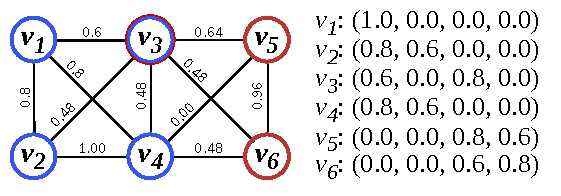
\includegraphics[width=0.8\linewidth,page=1]{fig/pictures.pdf}
  \caption{Running example with vector attributes and edge similarities.}
  \Description{Two overlapping four-vertex cliques with six vector-labeled vertices and pairwise similarity labels.}
  \label{fig:example}
\end{figure}

\begin{example}
  \label{ex:msc}
  Figure~\ref{fig:example} shows a vector-attributed graph with six vertices.
  Edge labels give the precomputed pairwise similarities.
  With threshold $\tau=0.6$, consider the two structural cliques
  \begin{align*}
    M_1&=\{v_1,v_2,v_3,v_4\}, &
    M_2&=\{v_3,v_4,v_5,v_6\}.
  \end{align*}

  Let $C_1=\{v_1,v_2,v_3,v_4\}$, $C_2=\{v_3,v_5,v_6\}$, and
  $C_3=\{v_3,v_4,v_5,v_6\}$. Their total and average similarities are
  \begin{align*}
    \simsum(C_1)&=4.16, & \avgsim(C_1)&\approx0.693\geq\tau,\\
    \simsum(C_2)&=2.08, & \avgsim(C_2)&\approx0.693\geq\tau,\\
    \simsum(C_3)&=2.56, & \avgsim(C_3)&\approx0.427<\tau.
  \end{align*}
  Thus $C_1$ and $C_2$ are $\tau$-semantic cliques, whereas the structurally valid
  clique $C_3$ is not.

  Moreover, neither $C_1$ nor $C_2$ has a strict superset that is a
  $\tau$-semantic clique, so both are MSCs.
\end{example}

\stitle{Problem Statement.}
\begin{problem}[MSC Enumeration]
Given a vector-attributed graph $\mathcal{G}=(V,E,\mathbf{X})$ and a threshold
$\tau \in [-1,1]$, enumerate all MSCs of $\mathcal{G}$.
\end{problem}


\subsection{Challenges}
\label{sec:challenges}
\stitle{Hardness.}
MSC enumeration contains classical MCE as a special case.  When singleton
outputs are excluded and $\tau$ does not exceed the minimum similarity on any
edge, every structural maximal clique of size at least two satisfies the
semantic constraint, so the $\Omega(3^{n/3})$ output lower bound carries over.
The associated decision problem is NP-complete.
\begin{theorem}
  \label{thm:np-complete}
Given $\mathcal{G}=(V,E,\mathbf{X})$, threshold $\tau\in[-1,1]$, and integer $k$,
  deciding whether an MSC of size $\geq k$ exists is \emph{NP-complete}.
\end{theorem}
\begin{proof}
  \textit{NP membership.}  The decision instance is positive if and only if
  it contains a $\tau$-semantic clique $C$ of size at least $k$.  The
  forward implication is immediate.  For the reverse implication, the finite
  family of feasible clique supersets of $C$ contains an inclusion-wise
  maximal member, whose size is at least $|C|\geq k$.  A certificate therefore
  need only provide such a feasible clique $C$: verifying all edges and
  $\avgsim(C)\geq\tau$ takes $O(|C|^2)$ time. Accordingly, NP verification
  requires only this feasibility certificate. If maximality were tested
  separately, examining only single-vertex extensions would be insufficient
  under the non-monotone constraint.

  \textit{NP-hardness.}  We reduce from the \textsc{Clique} decision
  problem~\cite{karp1972}, which asks whether $G_0=(V,E)$ contains a
  clique of size $\geq k$.
  Assign $\mathbf{x}_v = \mathbf{e}_1$ to every vertex, so
  $\mathrm{sim}(u,v) = 1$ for every edge, and set $\tau = 1$.
  Under this assignment $\avgsim(C) = 1 \geq \tau$ for every clique $C$,
  so every structural maximal clique is an MSC and vice versa.
  Any clique of size $\geq k$ in $G_0$ is contained in some structural
  maximal clique of size $\geq k$, which is also an MSC of size $\geq k$.
  Conversely, any MSC of size $\geq k$ is a clique of size $\geq k$
  in $G_0$.  Hence a size-$k$ MSC exists if and only if $G_0$ contains
  a clique of size $\geq k$, completing the reduction.
\end{proof}

The output sets of MSC enumeration and MCE are incomparable: a structural
maximal clique with $\avgsim(M)<\tau$ may contain semantically maximal subsets
that MCE never generates, while valid MSCs need not be structurally maximal.
Therefore, enumerating structural maximal cliques and retaining only those that
pass the average constraint is incomplete because an MSC need not be structurally maximal.
The output size, and hence the computational cost, follows the
threshold-dependent behavior characterized below.

\stitle{Output Distribution and Practical Scope.}
The number and sizes of MSCs vary substantially with $\tau$. At low thresholds,
the output approaches classical MCE. As $\tau$ increases, infeasible structural
cliques can fragment into many incomparable feasible sub-cliques, inflating both
the output and the unavoidable enumeration cost. At selective thresholds, most
cliques become infeasible and the output contracts. Because these transitions
depend on each dataset's similarity distribution, Section~\ref{sec:exp} uses a
fixed grid of edge-similarity quantiles rather than runtime-selected absolute
thresholds.

\stitle{Non-monotonicity and Framework Incompatibility.}
The core difficulty is that $\avgsim$ is non-monotone over the subset lattice.
In classical MCE, structural feasibility is monotone and maximality is enforced
implicitly by the $P=\emptyset$ invariant at every leaf, so the set of feasible
extensions can be characterized solely by the current state of $C$.
Under the average constraint, no such invariant exists: a partial clique with
$\avgsim(C)<\tau$ may still grow into a valid MSC, while one with
$\avgsim(C)\geq\tau$ may admit no feasible extension. Furthermore, whether a
candidate vertex can participate in a valid extension depends on its accumulated
similarity to the current partial clique, which evolves throughout the recursion
and cannot be captured by structural conditions alone. As a result, the pruning mechanisms based on structural monotonicity
lose their foundation, and the pivot strategy no longer applies.
A direct BK adaptation must therefore retain structurally valid intermediate
states even when they are currently infeasible. In the baseline developed
next, $\tau$ validates terminal semantic candidates but does not reduce the
structural recursion itself.


\section{Framework}

\stitle{Framework Overview.}
\semBK\ is a direct BK baseline that retains degeneracy-ordered $(P,X)$
recursion while omitting the structurally justified pivot. At each leaf, a
secondary \textsc{Check} pass over $X$ enforces inclusion-wise semantic
maximality.

\begin{algorithm}[t]
  \small
  \caption{Semantic BK with Check}
  \label{alg:semantic-max-clique}
  \SetKwFunction{FSearch}{Search}
  \SetKwProg{Fn}{Function}{:}{}

  \textbf{Input}: $G=(V,E)$, semantic vectors $\{\mathbf{x}_v\}$, threshold $\tau$\\
  \textbf{Output}: All MSCs $\mathcal{R}$

  Precompute $\mathrm{sim}(u,v)$ and degeneracy ordering $\sigma$\;
  Each worker initializes a private result set $\mathcal{R}_t\leftarrow\emptyset$\;
  \For{each $v \in \sigma$ \textbf{in parallel}}{
    $P \leftarrow \{u \in N(v) \mid \sigma(u) > \sigma(v)\}$\;
    $X \leftarrow \{u \in N(v) \mid \sigma(u) < \sigma(v)\}$\;
    \FSearch{$C=\{v\}, s_C=0, P, X, \textit{mode}=\mathrm{ENUM}, 0$}
  }
  \Return $\bigcup_t\mathcal{R}_t$\;

  \BlankLine
  \Fn{\FSearch{$C, s_C, P, X, \textit{mode}, k_{\min}$}}{
    $k \leftarrow |C|,\ \textit{hasFeasibleDesc} \leftarrow \mathbf{false}$\;
    $Q\leftarrow P$\;
    \For{each $v \in Q$}{
      $s_D \leftarrow s_C + \sum_{u\in C}\mathrm{sim}(u,v)$\;
      $P \leftarrow P \setminus \{v\}, P' \leftarrow P \cap N(v), X' \leftarrow X \cap N(v)$\;
      $\textit{res} \leftarrow$ \FSearch{$C \cup \{v\}, s_D, P', X', \textit{mode}, k_{\min}$}\;

      \If{$\textit{res}$}{
        $\textit{hasFeasibleDesc} \leftarrow \mathbf{true}$\;
        \lIf{$\textit{mode} = \mathrm{CHECK}$}{\Return \textit{true}}
      }
      $X \leftarrow X \cup \{v\}$\;
    }

    \If{$\neg \textit{hasFeasibleDesc}$}{
      \lIf{$k \geq 2 \land s_C < \tau\binom{k}{2}$}{\Return \textit{false}}
      \lIf{$\textit{mode} = \mathrm{CHECK}$}{\Return $k > k_{\min}$}

      \If{$X \neq \emptyset$}{
        \If{\FSearch{$C, s_C, X, \emptyset, \mathrm{CHECK}, k$}}{
          \Return \textit{true}\;
        }
      }

      \lIf{$k\geq2$}{$\mathcal{R}_t\leftarrow\mathcal{R}_t\cup\{C\}$}
      \Return \textit{true}\;
    }
    \Return $\textit{hasFeasibleDesc}$\;
  }
\end{algorithm}

\begin{figure}[!htb]
  \centering
  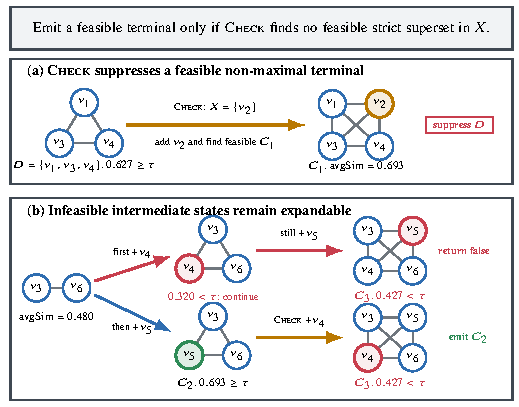
\includegraphics[width=0.95\linewidth]{tex-data/fig/sembk_graph_workflow.pdf}
  \caption{Selected \semBK\ branches on the running example.}

  \Description{Graph states on selected semantic BK branches, showing an exclusion-set check that suppresses a feasible non-maximal terminal and an infeasible intermediate state that remains expandable.}
  \label{fig:alg1}
\end{figure}

Figure~\ref{fig:alg1} exposes the graph states behind both terminal decisions.
In Figure~\ref{fig:alg1}(a), the feasible terminal
$D=\{v_1,v_3,v_4\}$ has $X=\{v_2\}$; \textsc{Check} reconstructs the feasible
strict superset $C_1$ and suppresses $D$. Figure~\ref{fig:alg1}(b) follows the
$v_6$-owned branch from $C=\{v_6,v_3\}$. The first insertion, $v_4$, remains
infeasible even after adding $v_5$. After backtracking, inserting $v_5$ yields
$C_2$ with $v_4$ in its exclusion set. \textsc{Check} reaches infeasible $C_3$,
returns false, and the outer search emits $C_2$.

\stitle{Degeneracy-Root Ownership.}
Degeneracy ordering assigns each clique to its earliest vertex under $\sigma$: later
neighbors form $P$, and earlier neighbors form $X$. This unique seed owns every
clique, including each MSC, while bounding the initial candidate set by graph
degeneracy.

\stitle{Terminal Feasibility and Maximality Check.}
The Boolean return value records whether a subtree contains a feasible
terminal. Only when no child reports one does $C$ become a candidate; an
infeasible candidate is discarded. A feasible candidate can still have a
strict extension through $X$, so \textsc{Check} searches that exclusion set
and suppresses $C$ upon finding one. The parameter $k_{\min}=|C|$ enforces
strict containment because the check recursion may also revisit sets no larger
than $C$.

\stitle{Why pivoting is not used.}
In standard BK, a pivot $p\in P\cup X$ guarantees that each structural maximal
clique in the current branch contains either $p$ or a vertex in
$P\setminus N(p)$.  Hence vertices in $P\cap N(p)$ need not become expansion
roots.  This argument depends on structural feasibility being preserved when
an adjacent pivot is added.

The average constraint invalidates that implication.  Consider a complete
graph on $\{s,p,u,w\}$ at the BK state $C=\{s\}$,
$P=\{p,u,w\}$, and $X=\emptyset$.  Let the three similarities within
$\{s,u,w\}$ equal $0.9$, the three similarities incident to $p$ equal $0$,
and $\tau=0.6$.  Then $\{s,u,w\}$ is an MSC with average $0.9$, whereas its
only strict clique superset has average $0.45$.  Choosing $p$ as the pivot
leaves only $p$ in $P\setminus N(p)$, so every explored child contains $p$
and the valid MSC $\{s,u,w\}$ is lost.  Pivot-free branching is therefore
required for the direct semantic BK baseline.

\stitle{Complexity.}
\begin{theorem}[Time and Space Complexity]
  \label{the:alg1complexity}
  Let $d_G$ be the degeneracy of $G$, let $\mathcal{L}$ be the feasible
  terminal states reached by the outer search, and let $X_C$ be the candidate
  set examined by \textsc{Check} for $C\in\mathcal{L}$.  The running time is
  $O^*(n2^{d_G}+\sum_{C\in\mathcal{L}}2^{|X_C|})$, where $O^*$ suppresses
  polynomial set-intersection costs.  A graph-independent upper bound is
  $O^*(3^n)$. With $T$ workers, the implementation uses
  $O(m+nD+Tn^2)$ worst-case space.
\end{theorem}
\begin{proof}
  A degeneracy seed has at most $d_G$ later neighbors.  Without pivoting, its
  outer recursion may visit every subset of those neighbors, giving
  $O^*(n2^{d_G})$ states.  For a feasible terminal $C$, \textsc{Check} may
  independently visit every subset of $X_C$.  The same earlier extension can
  be reconsidered for several terminals; charging a state to a pair of nested
  vertex sets gives the safe $O^*(3^n)$ bound.  Similarities and sparse
  adjacency require $O(m+nD)$ storage.  Each worker owns an $O(n)$
  accumulator, while decreasing candidate arrays retained by a worst-case
  \textsc{Check} stack total $O(n^2)$.
\end{proof}
For comparison, degeneracy-oriented pivoted MCE has the time
bound~\cite{eppstein2010,eppstein2013}
\[
O(d_Gn3^{d_G/3})
\]
The average constraint introduces more than an $O(|C|^2)$ validation cost:
valid MSCs may
occur at nonmaximal structural states, so the direct search may inspect all
$2^{d_G}$ subsets below a seed and revisit earlier-neighbor subsets in
\textsc{Check}. This gap formalizes the additional search complexity relative
to structural MCE.

\stitle{Design Implication.}
\semBK\ is a direct same-definition baseline that uses local search state and
no global visited table. Its pivot-free main search cannot prune every
infeasible intermediate, while \textsc{Check} may revisit earlier-neighbor
subspaces. Section~\ref{sec:algorithms} addresses these costs with two search
organizations tailored to different threshold regimes.


%%-------------------------------------------------------------------
\section{Proposed Algorithms}
\label{sec:algorithms}
This section presents two exact algorithms for complementary threshold regimes.
\subEnum\ decouples structural enumeration from semantic subset processing,
retaining Tomita pivoting and using admissible size-layer bounds. \monoSemMCE\
uses canonical reverse search, allowing $\tau$ to reject infeasible child
states before recursion. We evaluate both methods on the same quantile grid:
\subEnum\ provides broad threshold coverage, while \monoSemMCE\ targets
selective high-$\tau$ workloads.

%%-------------------------------------------------------------------
\subsection{\subEnum: Structural Decomposition and Subset Enumeration}
\label{sec:strsub}

\stitle{Structural--Semantic Decoupling and Containment.}
\subEnum\ restores the Tomita pivot by separating structural enumeration from
semantic subset search. Pivoted BK first produces structural maximal cliques;
the average constraint is then evaluated only within each resulting host.
Lemma~\ref{lem:containment} establishes that this separation preserves every
MSC.

For a host clique $M$ and target size $k$, let $\bar e_k$ be the mean of
the $\binom{k}{2}$ largest pairwise similarities in $M$. For each $v\in M$,
let $q_v(k)$ be the sum of its $k-1$ largest incident similarities within
$M$, and let $\bar q_k$ be the sum of the $k$ largest $q_v(k)$ values divided
by $k(k-1)$. Both quantities upper-bound the average similarity of any
size-$k$ subset; Properties~\ref{prop:topk} and~\ref{prop:vertexbound} prove
these bounds below.

\begin{algorithm}[t]
  \small
  \caption{\subEnum: Structural Decomposition and Subset Enumeration}
  \label{alg:strsub}
  \SetKwFunction{FBK}{BK}
  \SetKwProg{Fn}{Function}{:}{}

  \KwIn{$G=(V,E)$, similarities $\{\mathrm{sim}(u,v)\}_{(u,v)\in E}$, threshold $\tau$}
  \KwOut{All MSCs $\mathcal{R}$}

  $\mathcal{F} \leftarrow \emptyset$\;
  \tcc{Pipelined structural MCE and semantic processing}
  Build degeneracy ordering $\sigma$\;
  \For{each $v \in \sigma$ \textbf{in parallel}}{
    $P \leftarrow \{u \in N(v) \mid \sigma(u) > \sigma(v)\}$\;
    $X \leftarrow \{u \in N(v) \mid \sigma(u) < \sigma(v)\}$\;
    Run $\FBK(\{v\},P,X)$ with the following callback at each leaf $M$\;
  }

  \tcc{Callback: intra-clique semantic enumeration}
  \For{each structural leaf $M$ produced by a worker}{
    \lIf{$\avgsim(M) \geq \tau$}{$\mathcal{F} \leftarrow \mathcal{F} \cup \{M\}$; \textbf{continue}}
    \tcc{Admissible layer bounds}
    Sort edges of $M$ by similarity descending\;
    $k^* \leftarrow \max\!\bigl\{k \in [2,|M|-1] \mid \bar{e}_k \geq \tau\bigr\}$\;
    \lIf{$k^*$ does not exist}{\textbf{continue}}
    $\mathit{lmax} \leftarrow \emptyset$;\quad $\mathit{umask} \leftarrow \mathbf{0}$\;
    \For{$k \leftarrow k^*$ \KwTo $2$}{
      Compute the vertex-contribution bound $\bar{q}_k$ for size $k$\;
      \lIf{$\bar{q}_k < \tau$}{\textbf{continue}}
      \For{each size-$k$ subset $S \subseteq M$}{
        \lIf{$(S \mathbin{\&}\ \mathit{umask}) = S$
          \textbf{ and } $\exists\, T \in \mathit{lmax} : S \subseteq T$}{\textbf{continue}}
        \If{$\avgsim(S) \geq \tau$}{
          $\mathit{lmax} \leftarrow \mathit{lmax} \cup \{S\}$\;
          $\mathit{umask} \leftarrow \mathit{umask} \mid S$\;
          $\mathcal{F} \leftarrow \mathcal{F} \cup \{S\}$\;
        }
      }
    }
  }

  \tcc{Phase 3: Exact global filter}
  Sort $\mathcal{F}$ by $|\cdot|$ descending; remove exact duplicates\;
  Initialize an empty inverted index $\mathit{inv}:v\mapsto\emptyset$\;
  $\mathcal{R} \leftarrow \emptyset$\;
  \For{each equal-size group $\mathcal{G}\subseteq\mathcal{F}$ in descending size}{
    \For{each $S\in\mathcal{G}$ \textbf{in parallel}}{
      $r \leftarrow \displaystyle\mathop{\arg\min}_{v \in S}\ |\mathit{inv}[v]|$\;
      Keep $S$ iff no $T$ referenced by $\mathit{inv}[r]$ satisfies $S\subsetneq T$\;
    }
    Insert every kept $S\in\mathcal{G}$ into $\mathcal{R}$ and $\mathit{inv}$\;
  }
  \Return $\mathcal{R}$\;
\end{algorithm}
\begin{figure}[!htb]
  \centering
  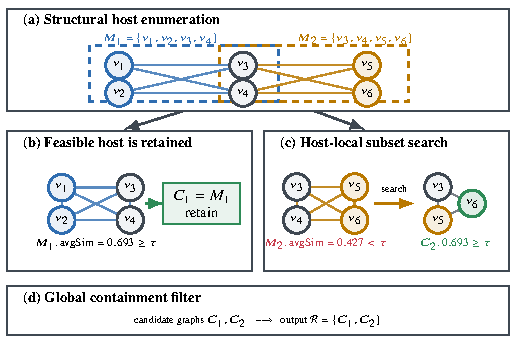
\includegraphics[width=0.95\linewidth]{tex-data/fig/strsub_graph_workflow.pdf}
  \caption{\subEnum\ execution on the running example.}



  \Description{Two overlapping structural maximal cliques shown as graphs, followed by direct retention of the feasible host, bounded subset search within the infeasible host, and global containment filtering.}
  \label{fig:alg2}
\end{figure}

Figure~\ref{fig:alg2}(a) first exposes the two overlapping structural hosts
$M_1=\{v_1,v_2,v_3,v_4\}$ and
$M_2=\{v_3,v_4,v_5,v_6\}$. The semantic phase handles each host
independently. Since $M_1$ satisfies the average constraint,
Figure~\ref{fig:alg2}(b) retains it directly as $C_1$. The infeasible $M_2$
instead activates the bounded subset search in Figure~\ref{fig:alg2}(c), which
recovers the feasible triangle $C_2=\{v_3,v_5,v_6\}$. The global containment
filter then removes duplicate candidates and strict subsets before returning
$\mathcal{R}=\{C_1,C_2\}$ (Figure~\ref{fig:alg2}(d)).


\begin{lemma}[Structural Superset of MSCs]
  \label{lem:containment}
  Every MSC is contained in at least one structural maximal clique of $G$.
  That is, for every MSC $C$, there exists a structural maximal clique
  $M$ such that $C \subseteq M$.
\end{lemma}

\begin{proof}
  By definition, every MSC is a clique of $G$.  Let $C$ be an arbitrary
  MSC, and consider the family
  \[
    \mathcal{F} = \{D \subseteq V \mid C \subseteq D \text{ and } D
    \text{ is a clique in } G\}.
  \]
  Since $C \in \mathcal{F}$, the family is nonempty.  Because $V$ is
  finite, $\mathcal{F}$ is finite, so we may choose a set $M \in
    \mathcal{F}$ that is maximal under inclusion.  By construction, $M$ is
  a clique containing $C$, and no vertex $w \in V \setminus M$ extends $M$
  to a larger clique; hence $M$ is a structural maximal clique of $G$,
  and $C \subseteq M$.
\end{proof}

\stitle{Structural Host Enumeration.}
Phase~1 uses degeneracy-oriented, pivoted
BK~\cite{tomita2006,eppstein2013} and is independent of $\tau$. Degeneracy roots
are dynamically scheduled; upon reaching a structural leaf $M$, the owning
worker immediately invokes the semantic callback instead of materializing the
complete family of structural maximal cliques.

\stitle{Bounded Semantic Subset Search.}
For each host $M$, Phase~2 visits subset sizes in descending order and uses a
host-local similarity matrix for repeated feasibility tests. The local filter
stores previously found feasible sets in $\mathit{lmax}$ and uses
$\mathit{umask}=\bigcup_{T\in\mathit{lmax}}T$ as a fast prerequisite for an
exact containment probe. If $S\subsetneq T$ for feasible $T$, then $S$ cannot
be an MSC; the filter therefore removes $S$ without changing the output. The
admissible bounds below skip entire size layers before subset generation.

\stitle{Global Maximality Reconciliation.}
An MSC may occur in multiple structural maximal cliques, so semantic subset
search may emit duplicate or subsumed candidates. Global reconciliation
consolidates them into $\mathcal{R}$. Candidates are deduplicated and processed
by decreasing size. For each $S$, the inverted index is probed through its
rarest vertex, limiting exact containment tests to retained supersets that
share that vertex. Equal-size queries read a frozen index in parallel and are
inserted only after the group completes. Because equal-size sets cannot
strictly contain one another and discarded supersets are covered transitively
by retained ones, this grouped procedure is equivalent to testing all larger
candidates.


\stitle{Admissible Size-Layer Bounds.}
Phase~2 as described iterates over all subset sizes from $|M|-1$ down
to $2$.  A key observation allows the starting size to be reduced: the
best achievable $\avgsim$ for any size-$k$ subset of $M$ is bounded
above by the mean of the $\binom{k}{2}$ largest pairwise similarities
in $M$.

\begin{property}[Sorted-Edge Upper Bound]
\label{prop:topk}
Let $e_1 \geq e_2 \geq \cdots \geq e_{\binom{m}{2}}$ be the pairwise
similarities of $M$ sorted in descending order.  For any size-$k$
subset $S \subseteq M$,
\[
  \avgsim(S) \;\leq\; \bar{e}_k
  \;:=\; \frac{1}{\tbinom{k}{2}} \sum_{i=1}^{\tbinom{k}{2}} e_i.
\]
\end{property}

\begin{proof}
Any size-$k$ subset $S \subseteq M$ uses exactly $\binom{k}{2}$ pairs,
each contributing at most the corresponding value in the sorted sequence
$e_1 \geq e_2 \geq \cdots$; hence $\simsum(S) \leq \sum_{i=1}^{\binom{k}{2}} e_i$,
and dividing both sides by $\binom{k}{2}$ gives the result.
\end{proof}

The sorted-edge bound ignores that its largest edges may be concentrated on
too few vertices to coexist in one size-$k$ subset. A complementary bound
tracks which vertices support those similarities. For each $v\in M$, let $q_v(k)$ be the
sum of the $k-1$ largest similarities between $v$ and vertices in
$M\setminus\{v\}$. Let $q_{(1)}(k)\geq\cdots\geq q_{(m)}(k)$ denote these
values in descending order.

\begin{property}[Vertex-Contribution Upper Bound]
\label{prop:vertexbound}
For any size-$k$ subset $S\subseteq M$,
\[
  \avgsim(S) \;\leq\; \bar{q}_k
  \;:=\; \frac{1}{k(k-1)}\sum_{i=1}^{k}q_{(i)}(k).
\]
\end{property}

\begin{proof}
For every $v\in S$, the sum of its similarities to the other vertices of
$S$ uses $k-1$ vertices from $M\setminus\{v\}$ and is therefore at most
$q_v(k)$. Summing
over $S$ counts each internal pair twice, so
\[
  2\simsum(S)
  \leq \sum_{v\in S}q_v(k)
  \leq \sum_{i=1}^{k}q_{(i)}(k).
\]
Division by $k(k-1)$ gives the claimed average-similarity bound.
\end{proof}

The prefix means $\bar e_k$ are non-increasing in $k$. The algorithm identifies
\[
  k^* = \max\!\bigl\{k \in [2, |M|-1] \;\big|\; \bar{e}_k \geq \tau\bigr\},
\]
and skips every larger layer. For each remaining $k$, it also skips the layer
when $\bar q_k<\tau$. Both bounds are admissible independently, so their joint
use cannot remove a feasible subset. Sorting the edge and per-vertex
similarity lists costs $O(m^2\log m)$ per host.

\stitle{Applicable Regime.}
\subEnum\ applies Tomita pivoting during structural MCE, whose cost is
$O(d_Gn\,3^{d_G/3})$ and independent of $\tau$.  At low thresholds, large
feasible subsets are identified early within each structural host.  At higher
  thresholds, the sorted-edge and vertex-contribution bounds skip infeasible size
layers.  Structural MCE remains a fixed phase cost, which motivates the
canonical search developed next for selective thresholds.

\stitle{Complexity.}
\begin{theorem}[Time Complexity of \subEnum]
  \label{the:alg2complexity}
  Let $\mathcal M$ denote the family of all structural maximal cliques of $G$.
  For each $M\in\mathcal M$, let $Q_M$ denote the number of exact local
  containment probes and let $b_M=\lceil |M|/w\rceil$ be its bitmap
  length in machine words.  \subEnum\ runs in
  \[
    \resizebox{0.99\columnwidth}{!}{$\displaystyle
      O\!\left(d_Gn\,3^{d_G/3}+\sum_{M\in\mathcal M}
      \left(2^{|M|}|M|^2+Q_Mb_M\right)
      +KN\log N+K\sum_{S\in\mathcal F}L_{\min}(S)\right)$}
  \]
  time, where $d_G$ is the degeneracy of $G$, $N=|\mathcal F|$ is the number
  of candidates before global deduplication,
  $K=\max_{S\in\mathcal F}|S|$, and
  $L_{\min}(S)=\min_{v\in S}|\mathit{inv}[v]|$.
\end{theorem}
\begin{proof}
  The structural phase uses degeneracy-oriented Tomita BK
  \cite{eppstein2013}, with cost $O(d_Gn\,3^{d_G/3})$. For a host $M$ of size $h$,
  subset enumeration visits at most $2^h$ subsets and evaluates each from the
  cached similarity matrix in $O(h^2)$ time.  Exact local maximality performs
  $Q_M$ bitmap containment probes of $b_M$ words each; keeping this term
  explicit also covers instances with many feasible local subsets.  The final
  filter sorts $N$ candidates in $O(KN\log N)$ time.  It then scans the shortest
  inverted list for each $S$, with at most $L_{\min}(S)$ sorted-set containment
  checks of $O(K)$ time.
\end{proof}

Within a host, non-monotone feasibility retains the exponential worst case;
the admissible bounds and local containment reduce inspected candidates without
changing the output.
\subsection{\monoSemMCE: High-$\tau$ Canonical Reverse Search}
\label{sec:monosem-mce}

\stitle{Motivation and Core Insight.}
Even with the size-layer bounds, \subEnum\ is bound to Phase~1: it enumerates
all structural maximal cliques before any semantic evaluation takes
place.  In the high-$\tau$ regime, the vast majority of structural
cliques may contain no feasible semantic result, yet each still contributes Phase~1
cost.  More fundamentally, the BK framework offers no mechanism to
incorporate $\tau$ into branching decisions---the threshold appears only
in validation, never in the search logic itself.  This structural
overhead motivates abandoning the BK skeleton entirely.

The obstacle to integrating $\tau$ directly into search is the
non-monotonicity of $\avgsim$: an infeasible clique can have a feasible
strict superset.  A search that retains only feasible states is therefore
complete only if every feasible target has a feasible construction path.
Theorem~\ref{thm:monotone} supplies such a path through the deletion rule defined next.

For a vertex $v$ in a clique $C$, define its \emph{similarity contribution}
as $a_C(v)=\sum_{u\in C\setminus\{v\}}\mathrm{sim}(u,v)$: the sum of its
similarities to the other vertices in $C$.  We delete a vertex with minimum
similarity contribution, breaking ties by vertex identifier.  The theorem
below proves that the remaining clique is feasible; the deterministic deletion
therefore defines the canonical parent used by reverse search.

The implementation traverses canonical trees by DFS from feasible edge roots.
It stores no complete size layer; a final containment filter enforces
inclusion-wise maximality.

\stitle{Feasible Parents and the Canonical Forest.}

\begin{theorem}[Feasible Minimum-Contribution Deletion]
  \label{thm:monotone}
  Let $C$ be a $\tau$-semantic clique of size $k\geq3$, with the
  similarity contribution $a_C(v)$ defined above.
  If $d(C)$ minimizes the pair $(a_C(v),v)$ lexicographically, then
  $C\setminus\{d(C)\}$ is a $\tau$-semantic clique.  Repeated application of
  this rule therefore reaches a feasible edge, and reversing these
  deletions gives a non-increasing-average insertion path.
\end{theorem}

\begin{proof}
  Each pair is counted once at each endpoint.  The minimum contribution
  therefore satisfies $a_C(d(C))\leq 2\simsum(C)/k$.  Deleting $d(C)$ leaves similarity sum
  at least $\simsum(C)(k-2)/k$, and hence
  \[
    \avgsim(C\setminus\{d(C)\})
    \geq
    \frac{\simsum(C)(k-2)/k}{\binom{k-1}{2}}
    =\avgsim(C)\geq\tau.
  \]
  Deterministic tie-breaking makes $d(C)$ unique.  Applying the same
  argument until two vertices remain preserves feasibility at every
  deletion; reversing the sequence proves the insertion-path claim.
\end{proof}

Define $p(C)=C\setminus\{d(C)\}$ for every feasible clique $C$ of size at
least three. The theorem makes $p(C)$ a feasible and unique parent, so all
feasible cliques form a forest rooted at feasible edges. This property does not
make arbitrary insertions or deletions monotone; it identifies one complete
feasible path for every target. \monoSemMCE\ traverses precisely these owned
parent--child edges and rejects alternative constructions before recursion.

Figure~\ref{fig:monotone} applies this rule to the running example. The upper
sequence constructs $C_1$ through canonical insertions. The lower panels
contrast the owned construction of $C_2$ with an alternative insertion that
forms the same clique but is rejected before recursion because the inserted
vertex is not $d(C_2)$.

\begin{figure}[t]
  \centering
  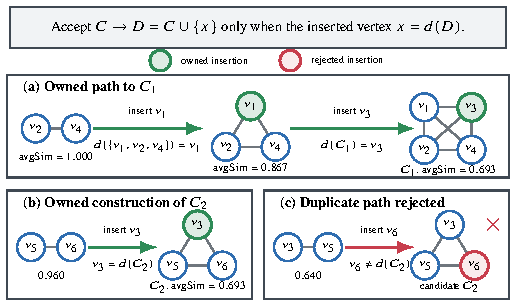
\includegraphics[width=0.95\linewidth]{tex-data/fig/monosem_graph_workflow.pdf}
  \caption{Canonical ownership on the running example.}
  \Description{Clique graphs illustrating the canonical-parent rule, the owned insertion paths to C1 and C2, and a duplicate construction of C2 rejected before recursion.}
  \label{fig:monotone}
\end{figure}

\begin{algorithm}[t]
  \small
  \caption{\monoSemMCE: Canonical Reverse Search}
  \label{alg:monosem-mce}
  \SetKwFunction{FSearch}{Search}
  \SetKwProg{Fn}{Function}{:}{}
  \textbf{Input}: $G=(V,E)$, semantic vectors $\{\mathbf{x}_v\}$, threshold $\tau$\\
  \textbf{Output}: All MSCs $\mathcal{R}$

  Precompute $\mathrm{sim}(u,v)$ for all $(u,v)\in E$\;
  $\mathcal{F} \leftarrow \emptyset$\;
  \For{each $(u,v)\in E$ with $u<v$ and $\mathrm{sim}(u,v)\geq\tau$
       \textbf{in parallel}}{
    $C\leftarrow\{u,v\}$; $s_C\leftarrow\mathrm{sim}(u,v)$\;
    $P\leftarrow N(u)\cap N(v)$\;
    $\acc[w]\leftarrow\mathrm{sim}(w,u)+\mathrm{sim}(w,v)$ for $w\in P$\;
    $a_C(u)=a_C(v)\leftarrow\mathrm{sim}(u,v)$\;
    \FSearch{$C,s_C,P,\acc,a_C$}\;
  }
  Apply Algorithm~\ref{alg:strsub}'s grouped strict-containment filter to $\mathcal{F}$, obtaining $\mathcal{R}$\;
  \Return $\mathcal{R}$\;
  \BlankLine
  \Fn{\FSearch{$C,s_C,P,\acc,a_C$}}{
    $k\leftarrow|C|$; $w_C\leftarrow s_C-\tau\binom{k}{2}$\;
    $\textit{hasValid}\leftarrow\textbf{false}$\;
    \For{each $v\in P$}{
      $\delta\leftarrow\acc[v]$\;
      \lIf{$w_C+\delta-\tau k<0$}{\textbf{continue}}
      $\textit{hasValid}\leftarrow\textbf{true}$\;
      $D\leftarrow C\cup\{v\}$\;
      Update $a_D$ from $a_C$ and $\mathrm{sim}(v,u)$ for $u\in C$\;
      \lIf{$v\neq\arg\min_{x\in D}(a_D(x),x)$}{\textbf{continue}}
      $P'\leftarrow P\cap N(v)$\;
      $\acc'[w]\leftarrow\acc[w]+\mathrm{sim}(w,v)$ for $w\in P'$\;
      \FSearch{$D,s_C+\delta,P',\acc',a_D$}\;
    }
    \lIf{\textbf{not} $\textit{hasValid}$}{$\mathcal{F}\leftarrow\mathcal{F}\cup\{C\}$}
  }
\end{algorithm}
\stitle{Feasible Edge Roots.}
Every feasible clique of size at least two reaches a feasible edge under
the deterministic deletion rule, so Algorithm~\ref{alg:monosem-mce} starts one tree
for each edge with similarity at least $\tau$.  A state stores the clique
  $C$, its pairwise sum $s_C=\simsum(C)$, the common-neighbor set $P$, candidate
accumulators $\acc$, and the member contributions $a_C$.  No BK exclusion set
is required: uniqueness follows from the canonical-parent test rather
than from an insertion order.

\stitle{Surplus and Canonical-Child Tests.}
For $k=|C|$ and $\delta=\acc[v]$, the extension satisfies
\[
  \W(C\cup\{v\})=\W(C)+\delta-\tau k.
\]
If this value is negative, the child itself is infeasible and cannot lie
on the canonical path of any feasible answer, so it is safely skipped.
For a feasible child $D=C\cup\{v\}$, the algorithm updates every member's
similarity contribution and accepts $D$ only if $v=d(D)$.  Equivalently, the canonical
parent of $D$ must be exactly $C$.  This test removes alternative
insertion paths before recursion rather than after state materialization.
The flag $\mathit{hasValid}$ is set before the ownership test because it records
the existence of any feasible one-vertex extension, not the existence of an
owned child. A state with such an extension cannot itself be inclusion-wise
maximal; the extension is generated from its unique canonical parent.

The canonical test removes duplicate insertion paths before recursion.
Accumulator values are restored during backtracking, so the result does not
depend on the order of floating-point additions.

\stitle{Inclusion-Wise Maximality.}
A state with no feasible single-vertex extension is added to
$\mathcal{F}$, but is not yet declared an MSC.  If such a candidate
$C$ is not inclusion-wise maximal, the finite family of feasible clique
supersets of $C$ contains an inclusion-wise maximal member $M$.  The
canonical search enumerates $M$ exactly once, and $M$ has no feasible
single extension, so it also belongs to $\mathcal{F}$.  The final
  grouped inverted-index containment filter consequently removes $C$.  Conversely,
an MSC is not contained in any other feasible candidate and is retained.

\begin{theorem}[Enumeration Correctness]
\label{thm:monosem-correctness}
Algorithm~\ref{alg:monosem-mce} generates every $\tau$-semantic clique
of size at least two exactly once and returns exactly all MSCs.
\end{theorem}
\begin{proof}
Existence follows by reversing the repeated deterministic deletions in
Theorem~\ref{thm:monotone}; every prefix is feasible and therefore passes
the surplus test.  Uniqueness follows because every non-root feasible
clique has the single parent $C\setminus\{d(C)\}$, and only that parent
accepts it as a child.  The preceding containment argument proves that
the final filter retains precisely the inclusion-wise maximal feasible
cliques.
\end{proof}


\stitle{Complexity.}
\begin{theorem}[Time and Space Complexity of \monoSemMCE]
  \label{thm:monosem-complexity}
  Let $F_\tau$ be the number of feasible cliques of size at least two, $K$ the
  maximum clique size, $\Delta$ the maximum degree, $T$ the number of workers,
  and $N=|\mathcal F|$ the number of terminal candidates.  A conservative
  bound for canonical search is
  \[
    O\!\left(F_\tau\Delta(\Delta+K\log\Delta)
      +KN\log N+K\sum_{S\in\mathcal F}L_{\min}(S)\right),
  \]
  with $O(m+T(n+K\Delta)+NK)$ words of space in addition to vector storage.
\end{theorem}
\begin{proof}
  Canonical ownership bounds accepted states by $F_\tau$.  A state tests at
  most $\Delta$ candidates.  For each candidate, common-neighbor intersection
  and accumulator maintenance cost $O(\Delta)$ conservatively, while updating
  and comparing at most $K$ member contributions uses cached similarities with
  $O(\log\Delta)$ lookup.  This is bounded by
  $O(\Delta(\Delta+K\log\Delta))$ per accepted state. The final filter has the
  same $O(KN\log N+K\sum_S L_{\min}(S))$ cost as in \subEnum.

  Sparse similarity adjacency and neighbor bitmaps use $O(m)$ words.  Each
  worker owns an $O(n)$ generation-tagged accumulator and $O(K\Delta)$ DFS
  scratch space.  Terminal candidates occupy $O(NK)$ words; no feasible-size
  layer or visited-state table is materialized.
\end{proof}

Canonical search is governed by the feasible-state family $F_\tau$ rather than
structural maximal cliques. This family can exceed the structural output at
intermediate thresholds but contracts sharply as $\tau$ becomes selective;
\subEnum\ instead continues to pay the structural MCE cost.
\section{Implementation}
\label{sec:opt}
All methods use a common C++17 loader, timing policy, and edge-similarity cache,
while their adjacency representation follows the access pattern of each search.
\StructBK\ and \subEnum\ repeatedly evaluate pivot neighborhoods and therefore
store each row as a sparse blocked bitmap: only nonempty 64-bit blocks are kept,
and intersections merge block identifiers before applying word-level AND.
\monoSemMCE\ retains the same representation for common-neighbor construction
at feasible edge roots. In contrast, the pivot-free \semBK\ scans its evolving
candidate and exclusion lists against sorted sparse adjacency rows; on these
short, irregular probes, constructing and searching block indices adds work.
The three semantic methods place vectors in a degree-descending breadth-first
layout for similarity-cache construction while preserving graph vertex IDs.

\stitle{Similarity Representation.}
Input vectors are normalized once into 64-byte-aligned float32 arrays, and
Advanced Vector Extensions~2 (AVX2) dot products populate the sparse
edge-similarity cache shared by all semantic methods. Similarity sums, semantic
surplus, and threshold products use double precision, and all algorithms apply
the same inclusive comparison
$\simsum(C)\geq\tau\binom{|C|}{2}$ and no method-specific tolerance. Within a
structural host $M$, \subEnum\ materializes an $|M|\times|M|$ float32 matrix so
that repeated subset tests avoid graph-level similarity lookups.
End-to-end timing includes this preprocessing, search, and result consolidation;
optional text serialization is disabled, while phase counters separately report
search work.

\stitle{Incremental Search State.}
\monoSemMCE\ maintains
$\acc[w]=\sum_{u\in C}\mathrm{sim}(u,w)$ because every child-feasibility test
reads this marginal contribution. Extending $C$ by $v$ updates only surviving
candidates as $\acc'[w]=\acc[w]+\mathrm{sim}(w,v)$, reducing an
$O(|P'|\,|C|)$ recomputation to $O(|P'|)$. Each worker owns a generation-tagged
array and reuses depth-indexed buffers; logical resets avoid clearing $O(n)$
entries, and backtracking restores modified values. \semBK\ instead computes
the marginal sum directly from $C$;
its terminal-only semantic test provides no pruning rule that would consume a
per-candidate accumulator. \subEnum\ evaluates semantic subsets against the
host-local float32 matrix and reuses its size-layer buffers.

\stitle{Parallel Ownership.}
OpenMP scheduling follows disjoint units already established by the algorithms.
\StructBK, \semBK, and \subEnum\ dynamically assign degeneracy roots to workers.
For a large fixed-size subset layer, \subEnum\ further partitions combinations
by their smallest selected vertex; workers read the frozen larger-size local
maxima and merge their same-size results after the layer. \monoSemMCE\ dynamically
assigns feasible edge roots, each of which owns one canonical tree. Mutable
recursion buffers, counters, and candidate output remain thread-local during
search.

\stitle{Result Consolidation.}
Both proposed methods use the grouped containment filter from
Algorithm~\ref{alg:strsub}. Candidates are sorted once by decreasing size and
deduplicated lexicographically. Queries within one equal-size group read a frozen
inverted index and run in parallel; retained candidates are inserted only after
the group completes. Consequently, synchronization occurs at result merging and
between size groups rather than on recursive search states.
\section{Experiments}
\label{sec:exp}

Seven research questions cover end-to-end efficiency and output agreement (RQ1),
threshold and graph-size scalability (RQ2--RQ3), parallelism and mechanisms
(RQ4--RQ5), the MSC output space (RQ6), and definition and pattern-family
comparisons (RQ7).

\subsection{Experimental Setup}
\label{sec:exp-setup}

\stitle{Methods and comparison scope.}
\StructBK\ implements BK with Tomita pivoting and degeneracy-ordered
roots~\cite{bron1973,tomita2006,eppstein2010,eppstein2013}; it supplies a
threshold-independent structural-time reference. \semBK\ is the direct
baseline: it uses the same MSC definition, threshold, similarity values, and
strict-containment filter as \subEnum\ and \monoSemMCE. Consequently, runtime
speedups are claimed only among these three exact MSC methods. \pairSim\ keeps
edges whose endpoint similarity reaches $\tau$ and then runs structural MCE; it
represents the every-pair similarity contract used by related constrained
enumeration models~\cite{yao2022similarbiclique}. FastQC enumerates maximal quasi-cliques under a degree-density
constraint~\cite{yu2023fastqc}, while FaPlex enumerates maximal $2$-plexes that
may omit one incident edge per vertex~\cite{zhou2020faplex}. These methods
define different pattern families and are used only for output-family
comparisons.
\stitle{Datasets.}
The evaluation contains three graphs with natural attributes and five public
graphs with reproducibly generated attributes. FB15K-237 descriptions use
all-MiniLM-L6-v2 embeddings; GitHub-Social uses its official 4,005-dimensional
developer features; and ogbn-arxiv retains its official 128-dimensional node
features~\cite{rozemberczki2021musae,toutanova2015observed,wang2020ogb}. For email-Enron and the four
SuiteSparse graphs~\cite{leskovec2014snap,davis2011uf}, the PCG64 pseudorandom
generator draws 256
coordinates independently from $U[-1,1)$ under fixed dataset seeds, followed
by $\ell_2$ normalization. Every graph topology is extracted directly from its
public source dataset. Generated vectors provide controlled inputs for runtime,
scale, and mechanism experiments; the semantic-output analyses in RQ7 use only
the two graphs with official natural attributes.

\begin{table}[t]
\footnotesize
\centering
\setlength{\tabcolsep}{3.6pt}
\begin{tabular*}{\linewidth}{@{\extracolsep{\fill}}lrrrl@{}}
\toprule
Dataset & $|V|$ & $|E|$ & $D$ & Attributes \\
\midrule
FB15K-237 & 14,541 & 248,611 & 384 & natural \\
GitHub-Social & 37,700 & 289,003 & 4,005 & natural \\
ogbn-arxiv & 169,343 & 1,157,799 & 128 & natural \\
email-Enron & 36,692 & 183,831 & 256 & generated \\
sc-nasasrb & 54,870 & 1,311,227 & 256 & generated \\
sc-pkustk11 & 87,804 & 2,565,054 & 256 & generated \\
sc-pwtk & 217,891 & 5,653,221 & 256 & generated \\
sc-ldoor & 909,537 & 20,770,807 & 256 & generated \\
\bottomrule
\end{tabular*}
\caption{Public graphs and vector attributes used in the evaluation.}
\label{tab:datasets}
\end{table}

\stitle{Protocol.}
Experiments run on an AMD Ryzen~9 7945HX workstation with 16 physical cores,
32 hardware threads, and 32\,GiB memory. We compile with GCC~13.2 and OpenMP.
Each process is limited to 16\,GiB and 32 OpenMP threads. The uniform timeout is
1,200 seconds. Completed runtime configurations are repeated three times and
reported by the median; time-limit exceeded (TLE) denotes one complete
1,200-second limit window.
Runtime binaries contain no statistics counters, and the reported in-memory
end-to-end time excludes optional text serialization.

Absolute cosine values are not comparable across vector sources. We therefore
derive thresholds from the edge-similarity distribution of each dataset. The
primary grid fixes $q_{20}$, $q_{80}$, and $q_{99}$ before execution; sensitivity
experiments use $q_{5}$, $q_{20}$, $q_{50}$, $q_{70}$, $q_{80}$, $q_{90}$,
$q_{95}$, $q_{97}$, and $q_{99}$.

\subsection{RQ1: Exactness and End-to-End Efficiency}
This experiment answers RQ1 by comparing complete MSC output sets and total
runtime across the 24 fixed dataset-threshold workloads. Exhaustive oracles first test 225,000
vertex-bound instances and 40,001 canonical-parent instances, including
negative similarities, equality at $\tau$, and tied minimum contributions.
On real graphs, jointly completed methods agree on normalized clique sets,
counts, and size histograms. In particular, all three exact methods return
263,721, 71,118, and 2,636 MSCs on GitHub-Social at $q_{20}$, $q_{80}$, and
$q_{99}$, respectively; \subEnum\ and \monoSemMCE\ also agree on every jointly
completed row of Table~\ref{tab:main-runtime}.
Across the eight graphs, the structural reference enumerates between 22,612 and 1,041,789 structural maximal cliques; these counts quantify the structural enumeration workload underlying the runtime comparisons.

\begin{table*}[t]
\scriptsize
\centering
\setlength{\tabcolsep}{2.5pt}
\renewcommand{\arraystretch}{1.02}
\begin{tabular*}{0.98\textwidth}{@{\extracolsep{\fill}}lrcrrrr@{}}
\toprule
Dataset & \shortstack{\StructBK\\structure} & $q$ & MSCs & \semBK & \subEnum & \monoSemMCE \\
\midrule
FB15K-237 & \multirow{3}{*}{0.103} & 20 & 206,470 & TLE & \cellcolor{bestgreen}\textbf{0.221} & TLE \\
 & & 80 & 76,106 & TLE & \cellcolor{bestgreen}\textbf{9.132} & TLE \\
 & & 99 & 7,476 & TLE & 45.234 & \cellcolor{bestgreen}\textbf{10.091} \\
\midrule
GitHub-Social & \multirow{3}{*}{0.110} & 20 & 263,721 & 34.777 & \cellcolor{bestgreen}\textbf{0.327} & 29.315 \\
 & & 80 & 71,118 & 27.548 & \cellcolor{bestgreen}\textbf{0.314} & 20.551 \\
 & & 99 & 2,636 & 21.495 & 0.391 & \cellcolor{bestgreen}\textbf{0.118} \\
\midrule
ogbn-arxiv & \multirow{3}{*}{0.309} & 20 & 925,239 & 1.590 & \cellcolor{bestgreen}\textbf{1.233} & 3.357 \\
 & & 80 & 226,936 & 1.165 & \cellcolor{bestgreen}\textbf{0.872} & 1.610 \\
 & & 99 & 10,261 & 1.249 & 0.843 & \cellcolor{bestgreen}\textbf{0.197} \\
\midrule
email-Enron & \multirow{3}{*}{0.090} & 20 & 223,703 & 9.196 & \cellcolor{bestgreen}\textbf{0.259} & 16.739 \\
 & & 80 & 60,352 & 8.312 & 1.266 & \cellcolor{bestgreen}\textbf{0.083} \\
 & & 99 & 1,819 & 4.084 & 0.206 & \cellcolor{bestgreen}\textbf{0.033} \\
\midrule
sc-nasasrb & \multirow{3}{*}{0.090} & 20 & 28,154 & TLE & \cellcolor{bestgreen}\textbf{0.301} & TLE \\
 & & 80 & 834,914 & TLE & 102.820 & \cellcolor{bestgreen}\textbf{0.759} \\
 & & 99 & 12,742 & TLE & 0.415 & \cellcolor{bestgreen}\textbf{0.079} \\
\midrule
sc-pkustk11 & \multirow{3}{*}{0.143} & 20 & 22,612 & TLE & \cellcolor{bestgreen}\textbf{0.645} & TLE \\
 & & 80 & 2,214,411 & TLE & TLE & \cellcolor{bestgreen}\textbf{2.219} \\
 & & 99 & 24,891 & TLE & 0.611 & \cellcolor{bestgreen}\textbf{0.167} \\
\midrule
sc-pwtk & \multirow{3}{*}{0.286} & 20 & 58,523 & TLE & \cellcolor{bestgreen}\textbf{1.093} & TLE \\
 & & 80 & 4,483,887 & TLE & TLE & \cellcolor{bestgreen}\textbf{3.977} \\
 & & 99 & 54,907 & TLE & 1.364 & \cellcolor{bestgreen}\textbf{0.421} \\
\midrule
sc-ldoor & \multirow{3}{*}{1.679} & 20 & 274,585 & TLE & \cellcolor{bestgreen}\textbf{4.870} & TLE \\
 & & 80 & 13,473,317 & TLE & 563.996 & \cellcolor{bestgreen}\textbf{14.944} \\
 & & 99 & 202,030 & TLE & 4.845 & \cellcolor{bestgreen}\textbf{1.658} \\
\bottomrule
\end{tabular*}
\caption{Median in-memory end-to-end runtime across 24 dataset-threshold workloads.}
\label{tab:main-runtime}
\end{table*}

Table~\ref{tab:main-runtime} shows that \subEnum\ completes 22 of 24 workloads
and every $q_{20}$ row, while \monoSemMCE\ resolves the two intermediate rows
where host-clique subset enumeration reaches TLE. At $q_{99}$, canonical search
is faster on all eight graphs, with speedups from $2.92\times$ on sc-ldoor to
$6.24\times$ on email-Enron. \semBK\ completes all nine rows on GitHub-Social,
ogbn-arxiv, and email-Enron but reaches TLE on all three FB15K-237 rows; its pivot-free search is slower than the faster of
\subEnum\ and \monoSemMCE\ on every completed row. The \StructBK\ column is reported only to
separate structural enumeration cost from semantic processing. Its
$0.090$--$1.679$ second range is much smaller than the hardest semantic runs,
showing that the dominant work comes from enforcing average feasibility and
inclusion maximality within the structural search space. The jointly completed
rows therefore establish both exact output agreement and the intended division
of labor: structural decomposition is effective when entire host cliques or
large size layers can be resolved together, whereas canonical traversal is
effective after semantic selectivity has contracted the feasible-state forest.

\subsection{RQ2: Threshold Sensitivity}
This experiment varies semantic selectivity while holding each graph fixed, so
a reversal in runtime ordering can be attributed to the threshold-induced
search space. Figure~\ref{fig:threshold-runtime} uses the full fixed quantile
grid. On ogbn-arxiv, \subEnum\ remains between 0.843 and 1.233 seconds across
the sweep, whereas \monoSemMCE\ decreases from 3.357 seconds at $q_{20}$ to
0.435 at $q_{95}$ and 0.197 at $q_{99}$; the methods cross near $q_{95}$. On
sc-ldoor, \subEnum\ completes the low-threshold cases, but the intermediate
fragmentation region produces 66.6 million MSCs at $q_{70}$ and exhausts its
host-clique subset search. As $q$ increases further, infeasible insertions
truncate the canonical forest, and \monoSemMCE\ falls from 91.945 seconds at
$q_{70}$ to 1.658 seconds at $q_{99}$. These trajectories match the mechanisms
developed in Sections~\ref{sec:strsub} and~\ref{sec:monosem-mce}: \subEnum\ amortizes
decisions over structural hosts, while \monoSemMCE\ visits only feasible,
canonically owned states. TLE points are shown at the fixed limit and are not
interpolated.

\begin{figure}[t]
\centering
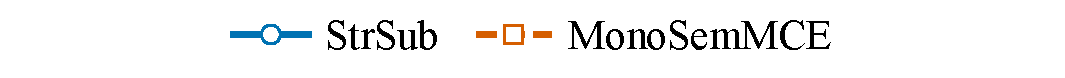
\includegraphics[width=0.72\linewidth]{tex-data/fig/threshold_runtime_legend.pdf}
\begin{subfigure}[t]{0.495\linewidth}
\centering
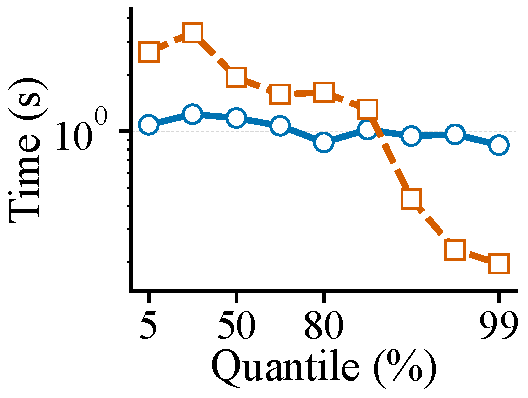
\includegraphics[width=\linewidth]{tex-data/fig/threshold_runtime_arxiv.pdf}
\caption{ogbn-arxiv}
\end{subfigure}\hfill
\begin{subfigure}[t]{0.495\linewidth}
\centering
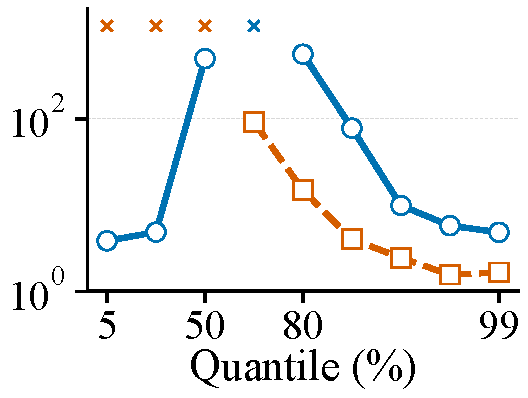
\includegraphics[width=\linewidth]{tex-data/fig/threshold_runtime_ldoor.pdf}
\caption{sc-ldoor}
\end{subfigure}
\caption{Threshold sweeps reveal complementary runtime regimes.}
\Description{Runtime over nine fixed threshold quantiles on ogbn-arxiv and sc-ldoor.}
\label{fig:threshold-runtime}
\end{figure}

\subsection{RQ3: Scalability with Graph Size}
Figure~\ref{fig:scale-runtime} reports absolute end-to-end runtime on shared
logarithmic axes as the graph
grows through nested induced ogbn-arxiv graphs whose vertices follow one fixed
degree order. The construction changes the number of vertices and outputs while
preserving the graph family and all six threshold quantiles. Both exact methods
remain executable across the four sizes: at $q_{20}$, \subEnum\ increases from
0.516 to 1.216 seconds and \monoSemMCE\ from 2.130 to 3.320 seconds; at
$q_{99}$, the corresponding increases are 0.340 to 0.707 and 0.057 to 0.200
seconds. Thus the experiment directly measures how each search organization
responds to graph growth, rather than treating one method as a universal
reference. Figure~\ref{fig:scale-regime} complements these absolute curves with
the runtime ratio across all size--threshold combinations. Its sign boundary
remains at $q_{95}$: \subEnum\ is faster through $q_{90}$, while
\monoSemMCE\ becomes faster at $q_{95}$ and $q_{99}$. The latter's $q_{99}$
advantage is $6.0\times$, $5.6\times$, $4.4\times$, and $3.5\times$ at 25K,
50K, 100K, and 169K vertices, respectively, so the selective-threshold benefit
persists as the graph grows by $6.8\times$.

\begin{figure}[t]
\centering
\begin{minipage}{0.85\linewidth}
\centering
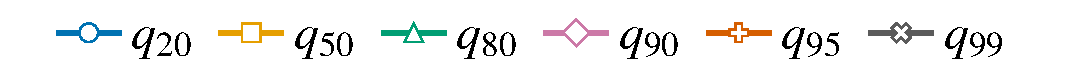
\includegraphics[width=0.94\linewidth]{tex-data/fig/scale_runtime_legend.pdf}
\begin{subfigure}[t]{0.495\linewidth}
\centering
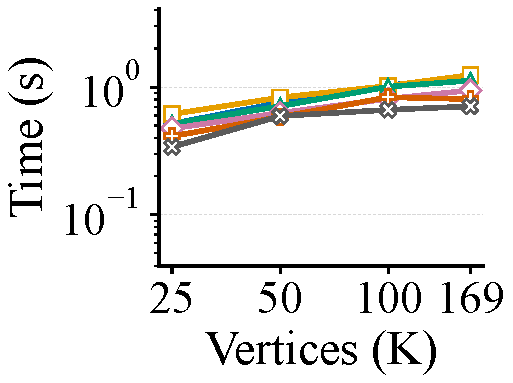
\includegraphics[width=\linewidth]{tex-data/fig/scale_runtime_strsub.pdf}
\caption{\subEnum}
\end{subfigure}\hfill
\begin{subfigure}[t]{0.495\linewidth}
\centering
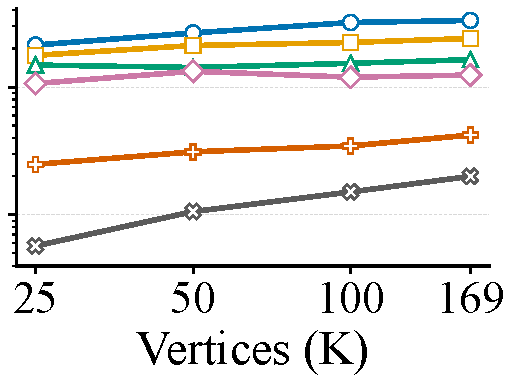
\includegraphics[width=\linewidth]{tex-data/fig/scale_runtime_monosem.pdf}
\caption{\monoSemMCE}
\end{subfigure}
\end{minipage}
\caption{Absolute runtime growth for both methods on logarithmic axes.}
\Description{End-to-end runtime of StrSub and MonoSemMCE over four nested graph sizes and six threshold quantiles.}
\label{fig:scale-runtime}
\end{figure}

\begin{figure}[t]
\centering
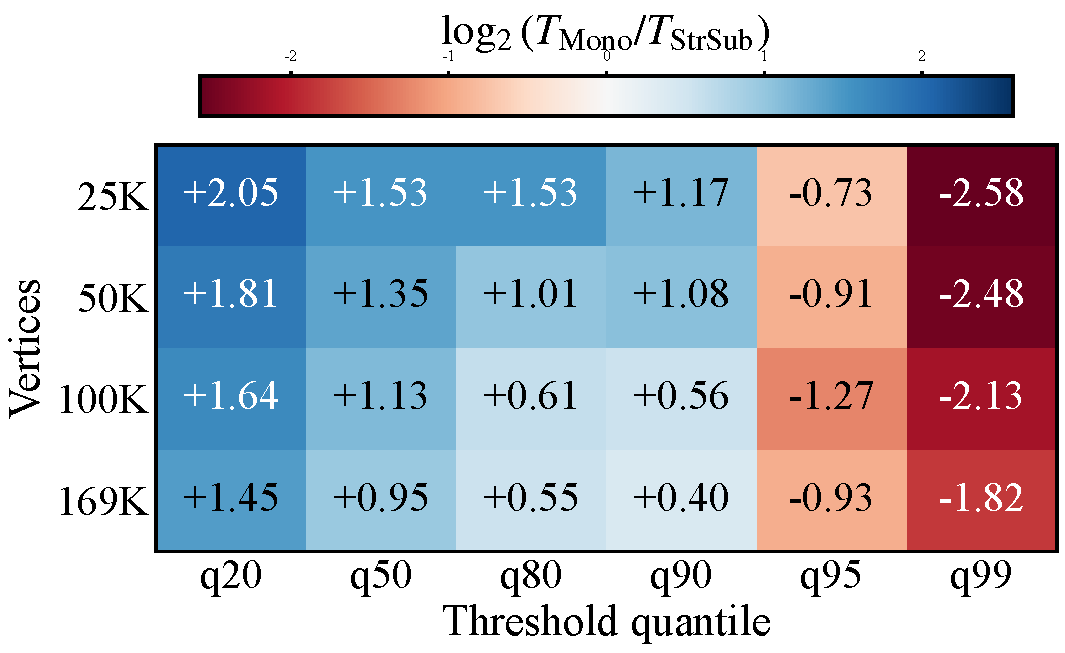
\includegraphics[width=0.75\linewidth]{tex-data/fig/scale_regime.pdf}
\caption{Relative runtime regimes remain stable across graph sizes.}
\Description{Log2 runtime ratio between MonoSemMCE and StrSub over four nested graph sizes and six threshold quantiles.}
\label{fig:scale-regime}
\end{figure}

\subsection{RQ4: Parallel Scalability}
Figure~\ref{fig:parallel-scaling} reports FB15K-237 at $q_{80}$ for \subEnum
and ogbn-arxiv at $q_{50}$ for \monoSemMCE. Dynamic edge-root scheduling reduces
\monoSemMCE\ from 13.054 seconds on one thread to 2.323 seconds on 32 threads,
a $5.62\times$ speedup. The gain continues from 16 to 32 threads because
canonical ownership exposes independent root subtrees without a shared visited
table. Fixed-size subset partitioning reduces \subEnum\ from 19.662 seconds to
8.232 seconds at 16 threads, a $2.39\times$ speedup, and reaches $2.26\times$
at 32 threads. Separately collected phase counters attribute 98.88\% of its
32-thread work to host-clique subset processing, while the final global filter
takes only 65 ms. The saturation therefore arises inside the dominant search
phase: structural maximal cliques induce tasks of unequal size, so a few large
hosts determine the completion time even though equal-size subsets within each
host are partitioned. The two curves consequently validate the parallelization
choices described in Section~\ref{sec:opt}: fine-grained canonical
roots provide more uniform concurrency than host-clique decomposition.

\begin{figure}[t]
\centering
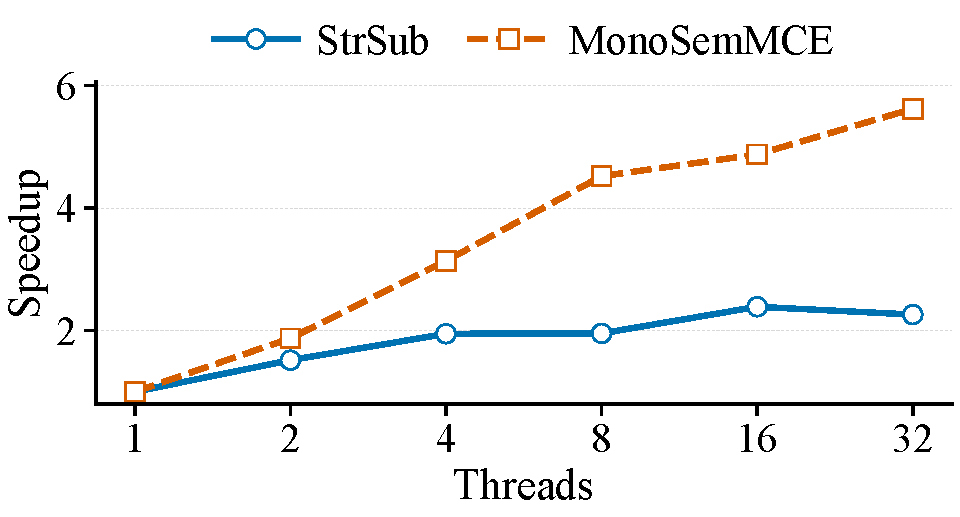
\includegraphics[width=0.80\linewidth]{tex-data/fig/parallel_scaling.pdf}
\caption{Parallel speedup under method-specific task scheduling.}
\Description{Speedup from one to 32 threads for StrSub on FB15K-237 at q80 and MonoSemMCE on ogbn-arxiv at q50.}
\label{fig:parallel-scaling}
\end{figure}

\subsection{RQ5: Search and Engineering Mechanisms}
Figure~\ref{fig:mechanisms} traces canonical-search diagnostics collected
outside timing runs. Accepted states contract from 17.08 million at $q_5$ to
18,011 at $q_{99}$. At the same time, canonical rejection accounts for 83.6\%
of candidate tests at $q_5$, whereas the $W$-based feasibility test prunes
86.1\% at $q_{99}$. Thus high selectivity reduces work before child-state
construction, matching the regime in which \monoSemMCE\ becomes dominant.
The ablations proceed hierarchically: they first
isolate semantic pruning in \subEnum, then duplicate-state organization in
\monoSemMCE, and finally two method-specific engine primitives while holding the
exact output fixed.

\begin{figure}[t]
\centering
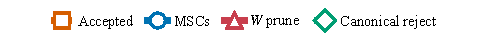
\includegraphics[width=0.96\linewidth]{tex-data/fig/mechanism_monosem_legend.pdf}
\begin{subfigure}[t]{0.495\linewidth}
\centering
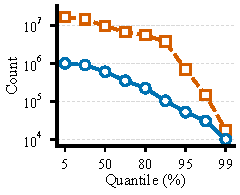
\includegraphics[width=\linewidth]{tex-data/fig/mechanism_monosem_states.pdf}
\caption{Search contraction}
\end{subfigure}\hfill
\begin{subfigure}[t]{0.495\linewidth}
\centering
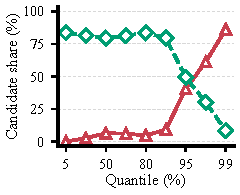
\includegraphics[width=\linewidth]{tex-data/fig/mechanism_monosem_rejections.pdf}
\caption{Candidate rejection}
\end{subfigure}
\caption{Canonical search contracts and shifts toward feasibility pruning.}
\Description{Accepted states and emitted MSCs, followed by the shares of candidate tests rejected by canonical ownership and the W-based feasibility test, over nine ogbn-arxiv thresholds.}
\label{fig:mechanisms}
\end{figure}

Table~\ref{tab:ablation} isolates the three \subEnum\ pruning mechanisms on
their appropriate metrics. On sc-nasasrb at $q_{99}$, the sorted-edge bound
reduces subset tests from 16.50 to 12.95 million, and the vertex bound reduces
them from 80.28 to 12.95 million. Local containment is measured separately on
FB15K $q_{80}$ because its primary effect is peak memory rather than subset-test
count, reducing 2.26 to 0.12~GiB.

\begin{table}[t]
\footnotesize
\centering
\setlength{\tabcolsep}{4.0pt}
\begin{tabular*}{\linewidth}{@{\extracolsep{\fill}}llrr@{}}
\toprule
Component & Metric / workload & Full & Removed \\
\midrule
Sorted-edge bound & tests (M) / nasa $q_{99}$ & \cellcolor{bestgreen}\textbf{12.95} & 16.50 \\
Vertex bound & tests (M) / nasa $q_{99}$ & \cellcolor{bestgreen}\textbf{12.95} & 80.28 \\
Local containment & GiB / FB15K $q_{80}$ & \cellcolor{bestgreen}\textbf{0.12} & 2.26 \\
\bottomrule
\end{tabular*}
\caption{Effect of the three \subEnum\ pruning mechanisms.}
\label{tab:ablation}
\end{table}

The corresponding runtimes are 0.287 versus 0.324 seconds for the sorted-edge bound,
0.287 versus 0.312 seconds for the vertex bound, and 8.060 versus 11.685
seconds for local containment. Every variant retains the same 12,742 outputs,
so the measured changes follow from pruning and local maximality checks while
preserving enumeration semantics. Table~\ref{tab:generation-ablation} then holds
the feasibility test, similarity cache, and final filter fixed while replacing
only duplicate-state organization. \emph{Visited DFS} suppresses duplicates
with a global state table, whereas \emph{Layered} materializes and deduplicates
all feasible cliques of one size before generating the next. Canonical ownership
is $4.2\times$--$6.3\times$ faster and uses $1.3\times$--$3.7\times$ less
memory than these alternatives across the two workloads. Every variant returns
the same normalized MSC set and size histogram, directly connecting the gain to
unique-parent state generation rather than feasibility pruning.

\begin{table}[t]
\footnotesize
\centering
\setlength{\tabcolsep}{4.0pt}
\begin{tabular*}{\linewidth}{@{\extracolsep{\fill}}lrrrr@{}}
\toprule
& \multicolumn{2}{c}{ogbn $q_{95}$} & \multicolumn{2}{c}{nasa $q_{80}$} \\
\cmidrule(lr){2-3}\cmidrule(lr){4-5}
Generation & s & GiB & s & GiB \\
\midrule
\rowcolor{bestgreen}Canonical & \textbf{0.388} & \textbf{0.39} & \textbf{0.729} & \textbf{0.22} \\
Visited DFS & 2.432 & 0.53 & 3.069 & 0.64 \\
Layered & 1.635 & 0.49 & 3.922 & 0.81 \\
\bottomrule
\end{tabular*}
\caption{Canonical ownership versus duplicate-state organizations.}
\label{tab:generation-ablation}
\end{table}

Table~\ref{tab:engineering-ablation} isolates the representation and state
updates selected for each search. Each row changes one choice while preserving
the remaining configuration; values are medians of three complete runs, and all
variants return identical counts. Sparse lists fit \semBK's irregular candidate
probes, while removing accumulator updates that its terminal-only test never
reads eliminates redundant work. Blocked bitmaps and vector reordering support
\subEnum's repeated pivot-neighborhood operations. For \monoSemMCE, incremental
accumulation directly supplies the marginal contribution used by every child
feasibility test. Complete results for all 31 evaluated configurations are
archived with the artifact.

\begin{table}[t]
\footnotesize
\centering
\setlength{\tabcolsep}{3.4pt}
\begin{tabular*}{\linewidth}{@{\extracolsep{\fill}}lllrrr@{}}
\toprule
Method & Workload & Choice & With (s) & Without (s) & Speedup \\
\midrule
\semBK & Enron $q_{80}$ & Sparse rows & 8.106 & 10.572 & $1.30\times$ \\
\semBK & Enron $q_{80}$ & Direct sum & 10.572 & 22.935 & $2.17\times$ \\
\subEnum & FB15K $q_{80}$ & Bitmap & 7.084 & 11.255 & $1.59\times$ \\
\subEnum & FB15K $q_{80}$ & Reorder & 7.084 & 8.792 & $1.24\times$ \\
\monoSemMCE & FB15K $q_{99}$ & Accumulator & 8.630 & 15.534 & $1.80\times$ \\
\bottomrule
\end{tabular*}
\caption{Paired engineering choices; other switches are fixed within each row, and speedup is without/with.}
\label{tab:engineering-ablation}
\end{table}

The paired speedups range from $1.24\times$ to $2.17\times$. More importantly,
they follow the access pattern of each algorithm: sparse rows and direct sums
avoid unused maintenance in \semBK, bitmap intersections and reordering serve
\subEnum's repeated neighborhood operations, and accumulators serve the
marginal tests performed at every \monoSemMCE\ insertion. The ablation therefore
supports method-specific engine configurations while keeping the mathematical
search procedures and outputs fixed.

\subsection{RQ6: MSC Output Space}
This experiment measures exact output counts and mean sizes on four graphs:
FB15K-237, ogbn-arxiv, sc-nasasrb, and sc-ldoor. It uses five quantiles from
$q_{20}$ through $q_{99}$. Figure~\ref{fig:result-distribution}
normalizes each value by \StructBK\ on the same graph. The geometric-mean count
ratios are 1.04, 7.50, 3.53, 0.61, and 0.11: intermediate thresholds split
large structural cliques into many feasible subsets that are maximal by
inclusion. Selective thresholds instead contract the result family. Mean size decreases
from 1.06 to 0.39 of the structural reference over the same grid. The count
peak and size decline describe the non-monotone search difficulty more precisely
than either statistic alone: one structural host can yield many smaller MSCs in
the intermediate regime, whereas high thresholds eliminate most extensions and
leave fewer, smaller outputs. This expansion--contraction pattern explains both
the intermediate \subEnum\ workload in RQ2 and the rapid contraction of the
\monoSemMCE\ state space at selective thresholds in RQ5.

\begin{figure}[t]
\centering
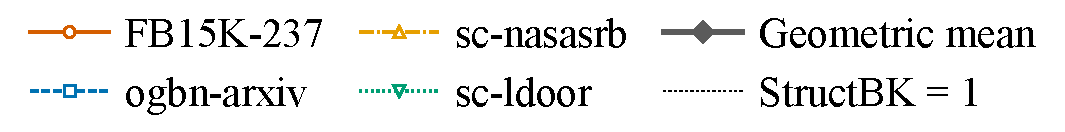
\includegraphics[width=0.94\linewidth]{tex-data/fig/result_distribution_legend.pdf}
\begin{subfigure}[t]{0.495\linewidth}
\centering
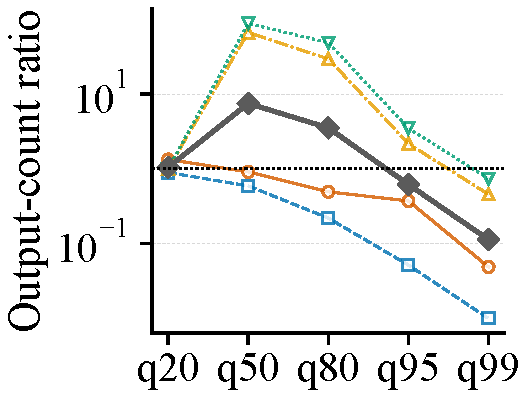
\includegraphics[width=\linewidth]{tex-data/fig/result_distribution_count.pdf}
\caption{Output count}
\end{subfigure}\hfill
\begin{subfigure}[t]{0.495\linewidth}
\centering
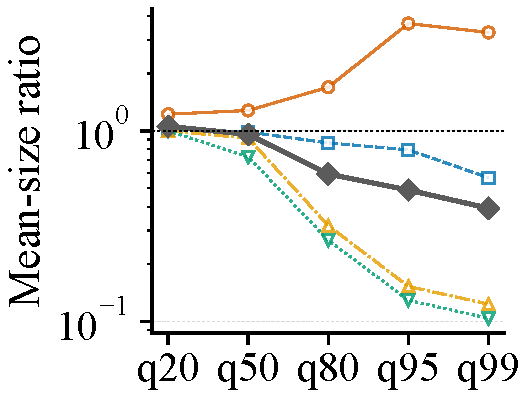
\includegraphics[width=\linewidth]{tex-data/fig/result_distribution_size.pdf}
\caption{Mean size}
\end{subfigure}
\caption{MSC output expands and then contracts as selectivity increases.}
\Description{Normalized MSC count and mean size over five threshold quantiles on four datasets.}
\label{fig:result-distribution}
\end{figure}

\subsection{RQ7: Group Preservation and External Pattern Families}
RQ7 first compares MSC with the every-pair definition. The reference cover
contains all size-at-least-ten MSCs at $q_{80}$ on GitHub-Social and the 25K
induced ogbn-arxiv graph used in RQ3; the response cover contains every non-singleton \pairSim\
output at the same $\tau$. For these overlapping covers, Extended B$^3$ Recall
is the overlap-aware, entity-level recall of the reference cover and measures
collective fragmentation~\cite{amigo2009bcubed}. Best-match recall
$R_{\max}(C)=\max_{P\in\mathcal P}|C\cap P|/|C|$ measures the largest
fraction of MSC $C$ retained by one
output~\cite{yang2013bigclam,hric2014recovery}.

Figure~\ref{fig:definition-recovery} shows the definition effect. \pairSim\
obtains B$^3$ Recall/best-match recall of 0.156/0.450 on GitHub-Social and
0.544/0.680 on ogbn-arxiv-25K. None of 605 GitHub-Social MSCs and only 0.32\%
of 624 ogbn-arxiv-25K MSCs is retained intact; respectively, 100\% and 84.9\%
lose at least 20\% of their members. The every-pair constraint therefore
fragments groups that remain complete and collectively feasible.

\begin{figure}[t]
\centering
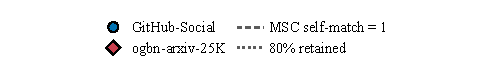
\includegraphics[width=0.94\linewidth]{tex-data/fig/definition_recovery_legend.pdf}
\vspace{-1.5ex}
\begin{subfigure}[t]{0.495\linewidth}
\centering
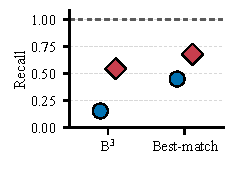
\includegraphics[width=\linewidth]{tex-data/fig/definition_recovery_summary.pdf}
\caption{Aggregate recovery}
\end{subfigure}\hfill
\begin{subfigure}[t]{0.495\linewidth}
\centering
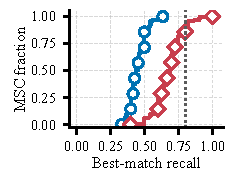
\includegraphics[width=\linewidth]{tex-data/fig/definition_recovery_cdf.pdf}
\caption{Per-group recovery}
\end{subfigure}
\caption{Pairwise thresholding fragments collectively feasible MSCs.}
\Description{The first panel compares Extended B-cubed and best-match recall
on two datasets; its dashed horizontal line is the MSC self-match reference.
The second panel shows cumulative distributions of best-match recall over
reference MSCs; its dotted vertical line marks 80\% retained.}
\label{fig:definition-recovery}
\end{figure}

A size-18 ogbn-arxiv MSC consists entirely of \texttt{cs.IT} papers on private
information retrieval. Its average is 0.919 at $\tau=0.889$, although 20 of 153
pairs fall below $\tau$. Thus 13.1\% of its within-group pairs violate the
every-pair threshold while the complete group remains collectively coherent;
this case instantiates the fragmentation measured by the cover-based metrics.

The external comparison fixes FastQC at $\gamma=0.9$, FaPlex at $k=2$, and
uses \StructBK as the structural reference on the same $q_{80}$ graphs. For two
groups $A$ and $B$, their match score is
$F_1(A,B)=2|A\cap B|/(|A|+|B|)$~\cite{yang2013bigclam}. \emph{Recovery}
averages each MSC's best match in the baseline family, whereas \emph{fidelity}
averages each baseline result's best match in the MSC family. This directional
pair measures output-family agreement rather than ground-truth clustering.

Figure~\ref{fig:external-quality} separates the two matching directions. The
left panel shows high MSC-to-baseline recovery on both datasets, whereas the
right panel shows substantially lower baseline-to-MSC fidelity. MSC self-matching
has score one by definition and appears only as the reference line. Recovery
spans 0.851--0.992, whereas fidelity spans 0.123--0.269. The high recovery follows
because every MSC is contained in some maximal clique, maximal quasi-clique, and
maximal 2-plex; fidelity exposes the additional patterns introduced by those extensions.
FastQC and FaPlex also differ from structural MCE: their mean induced edge densities
are 0.942--0.952, and fewer than 0.05\% of their outputs are cliques. Relative to
the MSC family, their result unions cover $12.5\times$--$27.6\times$ as many
distinct vertices and have lower mean pairwise cosine similarity.

\begin{figure}[t]
\centering
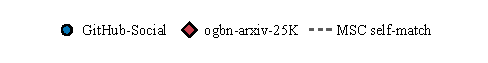
\includegraphics[width=0.94\linewidth]{tex-data/fig/external_recovery_legend.pdf}
\vspace{-1.5ex}
\begin{subfigure}[t]{0.495\linewidth}
\centering
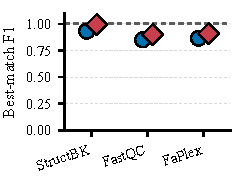
\includegraphics[width=\linewidth]{tex-data/fig/external_recovery_recovery.pdf}
\caption{MSC-to-baseline recovery}
\end{subfigure}\hfill
\begin{subfigure}[t]{0.495\linewidth}
\centering
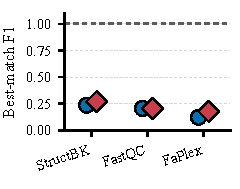
\includegraphics[width=\linewidth]{tex-data/fig/external_recovery_fidelity.pdf}
\caption{Baseline-to-MSC fidelity}
\end{subfigure}
\caption{Structural and relaxed families achieve high MSC recovery but lower family fidelity.}
\Description{Two dot plots separate MSC-to-baseline recovery from baseline-to-MSC fidelity for StructBK, FastQC, and FaPlex on two real graphs.}
\label{fig:external-quality}
\end{figure}

\section{Related Work}
\label{sec:related}

\stitle{Clique Enumeration and Listing.}
BK backtracking~\cite{bron1973}, Tomita pivoting~\cite{tomita2006}, and
degeneracy ordering~\cite{eppstein2010,eppstein2013} underpin exact MCE.
The classical output bound and reporting perspective were established by
Moon--Moser and subsequent maximal-clique analyses~\cite{moon1965,cazals2008}.
Recent methods reduce BK subproblems~\cite{deng2024rmce,wang2025hbbmc} or
summarize clique families~\cite{li2025cliquecomparator}; these methods preserve
structural maximality and do not impose a group-level vector constraint.
Large-graph implementations also exploit specialized search structures and
parallel execution~\cite{cheng2011,lessley2016,das2019}.

\stitle{Constrained Cohesive Subgraphs.}
FastQC~\cite{yu2023fastqc} and FaPlex~\cite{zhou2020faplex} enumerate maximal
quasi-cliques and $k$-plexes, respectively, while biplex methods relax complete
bipartite structure~\cite{dai2024biplex}. They change the adjacency contract,
whereas MSC retains a complete induced subgraph.

Earlier maximal similarity cliques threshold every pairwise similarity before
applying structural MCE~\cite{fang2013network}; this is the contract represented
by \pairSim\ in our evaluation. Average edge weight has also been used to select
one high-scoring structural maximal clique for short-text
segmentation~\cite{hua2015shorttext}. Fairness-aware MCE constrains counts or
balance among categorical vertex attributes~\cite{pan2022fairclique}. The MSC
contract enumerates all inclusion-wise maximal complete groups satisfying an
aggregate threshold over real-valued vectors.

The closest constrained-enumeration model is maximal similar-biclique
enumeration~\cite{yao2022similarbiclique}: its hereditary constraint requires
every vertex pair on one side to satisfy a similarity threshold. Similar-weight
bicliques likewise constrain edge weights in a bipartite
pattern~\cite{yang2025similarweight}. MSC differs along both axes: it operates on
cliques in a general graph and constrains the average of all pairwise vector
similarities. This aggregate condition admits low-similarity pairs and is
non-monotone under vertex insertion and deletion, which is precisely the source
of the search problem studied here.

\stitle{Attributed Community Search.}
Attributed-graph methods return partitions, such as
CODICIL~\cite{silva2012,zhou2009,ruan2013codicil}, or query-specific dense groups,
such as attributed truss communities~\cite{fang2016,huang2017}. Subspace and cross-graph variants likewise
optimize partition- or query-oriented
objectives~\cite{moser2009,gunnemann2010,fang2024iacs}. These tasks do not enumerate
inclusion-wise maximal complete groups under a vector aggregate, which gives MSC
a distinct enumeration contract.

\stitle{Vector Attributes.}
Representation models~\cite{bordes2013,sun2019,perozzi2014deepwalk,kipf2017}
can supply the vectors.
Given these fixed attributes, MSC evaluates the aggregate threshold exactly;
approximate vector retrieval addresses a separate nearest-neighbor
task~\cite{andoni2006,malkov2020,johnson2021}.
\section{Conclusion}
\label{sec:conclusion}
We formulated exact MSC enumeration under an average pairwise-similarity
constraint and showed that its associated size decision problem is NP-complete.
\subEnum\ combines structural decomposition with admissible semantic bounds;
\monoSemMCE\ turns feasible minimum-contribution deletion into a canonical
reverse-search forest. Their complementary threshold regimes jointly complete
all 24 fixed dataset--threshold workloads, with \monoSemMCE\
$2.92\times$--$6.24\times$ faster than \subEnum\ on every $q_{99}$ row.
Ablations connect these gains to layer pruning and canonical-state contraction,
while natural-attribute results show when averaging preserves complete groups
fragmented by pairwise thresholding. These results connect the group-level
semantic definition to complementary exact search organizations.
\bibliographystyle{ACM-Reference-Format}
\bibliography{references}

\end{document}
\endinput
